\begin{figure}[H]
	\centering
	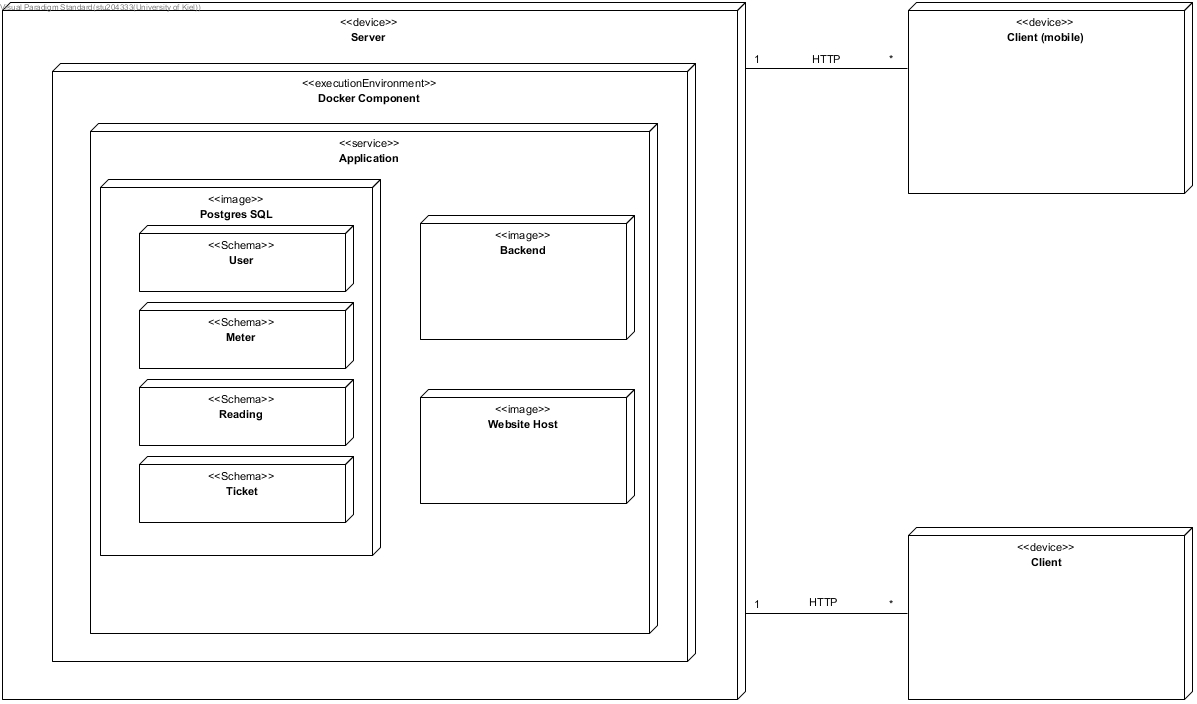
\includegraphics[width=16cm]{img/diagrams/DeploymentDiagram}
		\caption{Verteilungsdiagramm}
\end{figure}
Im Allgemeinen läuft die gesamte Software auf dem selben Server. Durch Docker werden einzelne Komponenten aber auf unterschiedliche Container aufgeteilt.\\
So läuft in einem Container die Software für das Backend, die über eine REST-API mit dem Frontend kommuniziert. Die Web und App Anwendungen können dann HTTP Anfragen an das Backend stellen.\\
Ein weiterer Container beinhaltet die SQL-Datenbank. Diese beinhaltet Schemata für Nutzer, Zähler, Zählerstände und Tickets.
